% SECTION 1.3 CHAPITRE 1 ACT1001
L'�quation de valeur (\emph{equation value}) sert � : 
\begin{itemize}
	\item{�galer, en valeur, des entr�es et sorties ;}
	\item{Comparer deux s�ries de flux mon�taires (\emph{Cash-flow}).}
\end{itemize}	
	
\begin{bcattention}
\textbf{Pour comparer, il faut tout �valuer au m�me moment dans le temps. Donc il faut actualiser et accumuler certains flux mon�taires.}
\end{bcattention}

\begin{bcattention}
\textbf{Pour tout mettre du m�me c�t� (`=0''), il faut pr�voir des signes diff�rents pour les d�p�ts et retraits.}
\end{bcattention}

\subsubsection{Exemple}
Pierre emprunte 1000\$ les 7, 14, 21 et 28 f�vrier. Il rembourse 1100\$ les 7,14,21 mars, puis r�gle sa dette en payant $X$ le 28 mars. Le taux d'int�r�t $i=8\%/$sem. Trouver X : 
\n
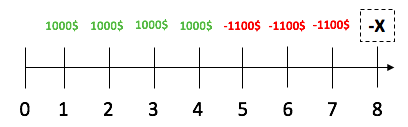
\includegraphics{equationvaleur.png}
\begin{gather*}
\green{1000\left( (1,08)^7 + (1,08)^6 + (1,08)^5 + (1,08)^5 \right)} - \red{1100 \left( (1,08)^3 + (1,08)^2 + (1,08)^1) \right)} -x = 0 \\
\text{etc...}
\end{gather*}

